\documentclass[11pt]{article}
\usepackage[margin=1in]{geometry}

% Packages we need
\usepackage{amsmath}
\usepackage{amsfonts}
\usepackage{mathtools}
\usepackage{amsthm}
\usepackage{float}
\usepackage{graphicx}
\usepackage{listings}
\usepackage{color} %red, green, blue, yellow, cyan, magenta, black, white
\usepackage{animate}
 \usepackage{tikz} 
\usepackage{pgfplots}
\pgfplotsset{width=10cm,compat=1.9}
\usepgfplotslibrary{external}
\tikzexternalize

% Header packages
\usepackage{fancyhdr}
\fancyhf{}
\pagestyle{fancy}


% Formatting document
\setcounter{secnumdepth}{0}
\setlength{\parindent}{0in}
\setlength{\parskip}{0.5em}

% MATLAB code
\definecolor{mygreen}{RGB}{28,172,0} % color values Red, Green, Blue
\definecolor{mylilas}{RGB}{170,55,241}

% Commands
\DeclarePairedDelimiter\ceil{\lceil}{\rceil}
\DeclarePairedDelimiter\floor{\lfloor}{\rfloor}
\newcommand{\ws}{\text{ }}
\newcommand{\e}[1]{\times 10^{#1}}

% Header
\lhead{\textsc{CS 5220 -- Project 1}} % TODO: enter title here
\rhead{\textsc{Junteng Jia -- jj585\\Sania Nagpal -- sn579\\Bryce Evans -- bae43}} % Authors
\setlength{\headheight}{0.5in}
\cfoot{\thepage}

% Title
\title{CS 5220 -- Project 2} %TODO: enter title here
\author{
  \begin{tabular}{l c l}
    Junteng Jia  & -- & jj585 \\
    Sania Nagpal & -- & sn579 \\
    Bryce Evans  & -- & bae43 \\
  \end{tabular}\\
  \rule{\linewidth}{0.4pt}
}
\date{}

\lstset
{
    frame=tb,
    language=C++,
    aboveskip=3mm,
    belowskip=3mm,
    showstringspaces=false,
    columns=flexible,
    basicstyle={\small\ttfamily},
    numbers=none,
    numberstyle=\tiny\color{gray},
    keywordstyle=\color{blue},
    commentstyle=\color{dkgreen},
    stringstyle=\color{mauve},
    breaklines=true,
    breakatwhitespace=true,
    tabsize=4
}

\begin{document}
    \thispagestyle{empty}
    \maketitle
    \begin{center}
        \animategraphics[autoplay, loop, height=15cm]{10}{dam_break-}{0}{50}
    \end{center}
    \begin{center}
    We did the domain decomposition for speed up and it works!
    \end{center}

    \clearpage
    
    \section{Our work}
        There are three major optimization base on the original code.
        \begin{enumerate}
            \item Profiling
            \item Parallelization
            \item Tuning
        \end{enumerate}
    
        \vspace{0.3cm}
                

        \subsection{Profiling}
        We did some hotspot analysis of the serial code, and this is what we find out:
        \begin{figure}[H]
            \centering
            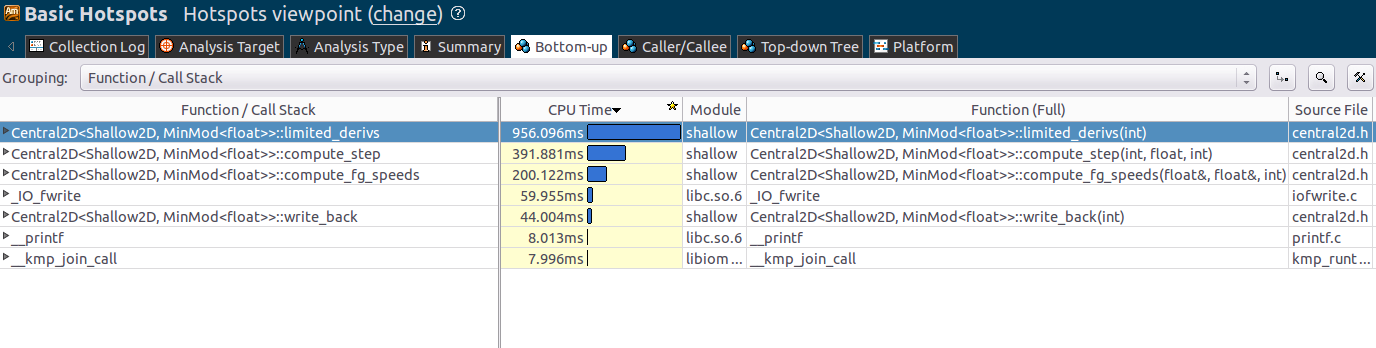
\includegraphics[width=4.5in]{hotspot.png}
            \caption{Hotspot analysis by amplxe-cl}
        \end{figure}
        
        We find that more 58\% of time is spent on the function call $"$limited\_derivs$"$. However, to our surprise, the function has been vectorized on assembly language level. We think since the data is not continuous in memory, there is a delay for acquiring data from memory to register. Probably that's why this function call is so slow. To further optimize this function call, we have to work on data dependence.

        \begin{figure}[H]
            \centering
            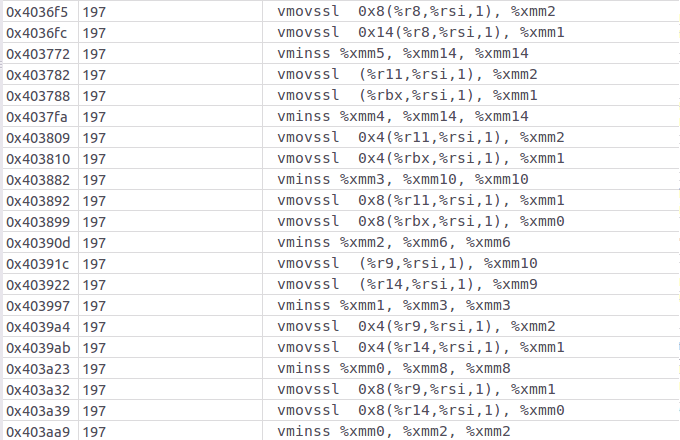
\includegraphics[width=4.5in]{assmbly.png}
            \caption{Assmbly for hotspot}
        \end{figure}

        \clearpage
        
    
        
        \subsection{Parallelization}
        We parallelized our code based on domain decomposition idea. The \texttt{-d} option specify how many time we split the domain along one direction. \\

        In our code, each pocessor has its own domain of simulation with \texttt{nghost} layer of ghost cells. We maintain an extra data structure \texttt{sg\_} for the whole simulation board. And there are three stages in each iteration of our parallel code:
        \begin{itemize}
            \item \texttt{Apply periodic}: In this stage, each thread copy the periodic boundary to their own ghost cells. After this stage, each one of those subdomains is ready for simulation.
            \item \texttt{Run step}: In this stage, each thread do simulation on their own subdomain, and the water height and water speed of each cell is updated.
            \item \texttt{Write back}: In this stage, every thread copy their updated subdomain back to the \texttt{sg\_} data structure. There is a barrier after this stage to make sure before next iteration, the data needed by ghost cells is up-to-date.
        \end{itemize}

        \begin{center}
			\begin{tikzpicture}
			\begin{axis}[
            title={},
            xlabel={Number of Processors},
            ylabel={Time per step (ms)},
            xmin=0, xmax=16,
			ymin=0, ymax=60,
			xtick={0,4,8,12,16},
			ytick={0,10,20,30,40,50,60},
			ymajorgrids=true,
			grid style=dashed,
			]
			
			\addplot[
			color=blue,
			mark=square,
			]
			coordinates {
			(1,59.2)(4,12.3)(9,6.0)(16,5.5)
			};
			\legend{Time}
			
			\end{axis}
			\end{tikzpicture}
        \end{center}
        \begin{figure}[H]
            \centering
            \caption{Strong Scaling}
        \end{figure}

        \begin{center}
			\begin{tikzpicture}
			\begin{axis}[
            title={},
            xlabel={Number of Processors},
            ylabel={Time per step (ms)},
            xmin=0, xmax=16,
			ymin=0, ymax=300,
			xtick={0,4,8,12,16},
			ytick={0,100,200,300},
			ymajorgrids=true,
			grid style=dashed,
			]
			
			\addplot[
			color=blue,
			mark=square,
			]
			coordinates {
			(1,43.8)(4,48.0)(9,98.4)(16,245)
			};
			\legend{Time}
			
			\end{axis}
			\end{tikzpicture}
        \end{center}
        \begin{figure}[H]
            \centering
            \caption{Weak Scaling}
        \end{figure}

    \section{Summary}
        
    Through this project:
    \begin{itemize}
        \item We analysed the hotspot of our code, yet we haven't done any tuning.
        \item Strong scaling for the parallel code is okey for the first three points, but the fourth point is bad.
        \item Weak scaling for the parallel code is okey for the first three points, but the fourth point is terrible.
    \end{itemize}

    In the furture:
    \begin{itemize}
    	\item We will try to cut down the time for calling \texttt{limited\_diffvs} by tuning.
    	\item We will use more layer of ghost cells and batch of steps simulations.
    	\item We will further optimize the code by hotspot analysis.
    \end{itemize}
\end{document}

